%% ============================================================================
%% FINAL MANUSCRIPT FOR EPIDEMICS SUBMISSION
%% ============================================================================

\documentclass[review, 12pt]{elsarticle}


% --- PACKAGES ---
\usepackage{lineno}
\usepackage{booktabs}
\usepackage{amsmath, amssymb}
\usepackage{graphicx}
\usepackage[margin=2.5cm]{geometry}

% Load hyperref late to avoid conflicts
\usepackage{hyperref}
% Strip elsarticle frontmatter commands from PDF metadata/bookmarks
\pdfstringdefDisableCommands{%
  \def\corref#1{}%
  \def\cnotenum{}%
  \def\@corref#1{}%
}

% --- BIBLIOGRAPHY STYLE ---
\bibliographystyle{elsarticle-num} 

\journal{Epidemics}

\begin{document}

\begin{frontmatter}

%% --- TITLE ---
\title{The Prevention Theorem: Time-Dependent Constraints on Post-Exposure Prophylaxis for HIV}

%% --- AUTHORS ---
\author[1,2]{A.C. Demidont, DO\corref{cor1}}
\ead{ac.demidont@nyxdynamics.com}

\address[1]{Independent Researcher}
\address[2]{Nyx Dynamics, LLC, 268 Post Rd. East, Fairfield, CT 06428, USA}

\cortext[cor1]{Corresponding author}

%% --- ABSTRACT ---
\begin{abstract}
Antiretroviral agents for HIV prevention are typically evaluated in terms of trial efficacy and programmatic coverage, but rarely in terms of whether they admit a true mathematical solution to prevention. Here we introduce the Prevention Theorem, which formalizes prevention for a given exposure e as the condition $R_0(e)=0$, meaning that the probability of establishing a productive, transmissible infection is exactly zero. Within this framework, post-exposure prophylaxis (PEP) is not delayed treatment but a time-dependent operator acting on within-host infection establishment dynamics. Using a mechanistic model of reservoir seeding and proviral integration, we derive the PEP Window Corollary: PEP can enforce $R_0(e)=0$ only when initiated within a finite biological window prior to irreversible integration and initial reservoir establishment. Beyond this window, all reachable system states satisfy $R_0(e)>0$ and are irreducible by post-exposure intervention. Parameterization using virological data indicates that this window extends to approximately 72 hours for mucosal exposures but is compressed to roughly 12–24 hours for parenteral exposures due to bypass of early immune bottlenecks. As an applied example, we show that structural access delays in high-risk populations—such as people who inject drugs—frequently exceed this compressed parenteral window. Consequently, for such exposures the condition $R_0(e)=0$ is mathematically and biologically unreachable before access is even attempted, rendering the failure of post-exposure prevention a consequence of violated biological boundary conditions rather than pharmacological efficacy.
\end{abstract}

%% --- KEYWORDS ---
\begin{keyword}
HIV prevention \sep Mathematical modeling \sep Prevention Theorem \sep PEP timing \sep Irreversible dynamics
\end{keyword}

\end{frontmatter}

%% --- HIGHLIGHTS ---
\section*{Highlights}
\begin{itemize}
    \item Prevention is defined mathematically as the condition $R_0(e)=0$.
    \item PEP operates as a time-dependent function racing against irreversible integration.
    \item A finite biological window exists beyond which prevention is mathematically impossible.
    \item Parenteral exposures compress this window to 12--24 hours, bypassing mucosal bottlenecks.
    \item Structural access delays in PWID invariably exceed this compressed biological limit.
\end{itemize}

\linenumbers

\section{Introduction}

Despite the availability of antiretroviral agents with trial efficacies approaching or exceeding 99\%, HIV prevention following exposure remains constrained by the biological dynamics of infection establishment \cite{grant_preexposure_2010, anderson_emtricitabine-tenofovir_2012}. Prevention is often discussed as a matter of coverage, adherence, or early treatment, implicitly assuming that post-exposure intervention remains feasible at all times following contact. A formal evaluation of this assumption requires specifying what prevention means in mathematical terms. Previous work has shown that HIV transmission and progression models are often highly sensitive to uncertain biological parameters, underscoring the difficulty of drawing robust conclusions from long-horizon simulations without strong constraints on initial conditions and system dynamics\cite{BlowerDowlatabadi1994}.

We define prevention for a specific viral exposure $e$ as the condition $R_0(e)=0$, corresponding to zero probability that the exposure establishes a productive, transmissible infection. Any state satisfying $R_0(e)>0$ admits non-zero onward transmission and therefore cannot be considered complete prevention. Within this formulation, pre-exposure prophylaxis enforces $R_0(e)=0$ by rendering the host non-susceptible prior to contact, whereas post-exposure prophylaxis (PEP) attempts to enforce $R_0(e)=0$ after contact but before infection establishment becomes irreversible.

Crucially, PEP operates as a time-dependent operator acting on within-host establishment dynamics, racing against irreversible biological processes including proviral integration and latent reservoir seeding. Once these processes are complete, the system undergoes a phase transition to an irreducible infection state in which $R_0(e)>0$ is permanently fixed, independent of subsequent therapeutic intervention \cite{mcmichael_immune_2010, wahl_hiv_2023, siliciano_enhanced_2015}. This formulation applies to any pathogen in which irreversible genomic integration or long-lived latent reservoirs fix infection status beyond a critical temporal threshold.

In the sections that follow, we formalize this constraint through the Prevention Theorem and its corollaries, derive the finite temporal window during which PEP can enforce prevention, and illustrate the consequences of violating this boundary condition using the structural context of injection drug use as an applied example.

\section{Methods}

\subsection{Theoretical Framework: The Prevention Theorem}

We define the state of true prevention for a specific viral exposure $e$ as the condition where the basic reproductive number for that exposure, $R_0(e)$, is exactly zero.

\begin{equation}
\text{Condition for Prevention: } R_0(e) = 0
\end{equation}

This condition implies that the probability of the exposure establishing a productive, transmissible infection is zero \cite{greenhalgh_mathematical_1997, liang_stochastic_2016}. Interventions are classified by their ability to enforce this condition. Pre-exposure prophylaxis (PrEP) enforces $R_0(e) = 0$ by rendering the host non-susceptible prior to contact. Post-exposure prophylaxis (PEP) attempts to enforce $R_0(e) = 0$ by extinguishing the virus after contact but before the infection becomes self-sustaining.

\subsection{Closed-Form Prevention Solution}

Let $R(t)$ denote the total number of infected cells resulting from a single exposure event at time $t$. The system admits exactly one closed-form prevention solution:

\begin{equation}
R(0) = 0 \;\Rightarrow\; R(t) = 0 \quad \forall t.
\end{equation}

If no infected cells exist at the initial condition, no infected cells can arise at any future time. For any initial condition satisfying $R(0) > 0$, no post-exposure or therapeutic intervention can mathematically guarantee $R(t)=0$; all such interventions act only on the subsequent trajectory of $R(t)$ and not on its initial condition \cite{grant_evidence_1987}.

\subsection{Infection Establishment Dynamics}

We model within-host establishment dynamics following a single exposure event using logistic formulations for reservoir seeding, $P_{\text{seed}}(t)$, and proviral integration, $P_{\text{int}}(t)$ \cite{mcmichael_immune_2010}. These functions describe the cumulative probability that irreversible biological transitions have occurred by time $t$.

\subsection{Master Equation for Time-Dependent Prevention}

The efficacy of post-exposure intervention is time-dependent. We define the reproductive number as a function of intervention timing:

\begin{equation}
R_0(e,t) = 1 - E_{\mathrm{PEP}}(t)
\end{equation}

with the efficacy function defined as:

\begin{equation}
E_{\mathrm{PEP}}(t) = (1 - P_{\text{seed}}(t))\,\varepsilon_{\max} + (P_{\text{seed}}(t) - P_{\text{int}}(t))\,\varepsilon_{\text{mid}} + P_{\text{int}}(t)\,\varepsilon_{\min}
\end{equation}

Here, $\varepsilon_{\max}$ represents efficacy prior to seeding, $\varepsilon_{\text{mid}}$ represents efficacy during the seeding window, and $\varepsilon_{\min}$ represents efficacy after integration is established (typically zero for prevention purposes). 

Because $E_{\text{PEP}}(t)$ depends on cumulative probabilities of irreversible biological transitions, once integration is established, this operator, $E_{\mathrm{PEP}}(t)\to 0$ and $R_0(e,t)$, admits a hard temporal cutoff once established.\cite{tanner_npep_2025}

\textbf{Corollary 1 (PEP Window Corollary):} \textit{Post-exposure prophylaxis can enforce the prevention condition $R_0(e)=0$ if and only if initiated within a finite biological window $t < t_{crit}$ prior to irreversible proviral integration. Beyond this critical threshold, all reachable system states satisfy $R_0(e)>0$ and are irreducible by post-exposure intervention or any therapeutic option currently available.}


\section{Results}

\subsection{Visualization of the Theorem}

Figure \ref{fig:theorem} illustrates the four core components of the Prevention Theorem. Panel A shows the timeline of infection establishment, with reservoir seeding preceding proviral integration. Panel B demonstrates the time-dependent efficacy function $E_{\mathrm{PEP}}(t)$, which decays monotonically toward zero as irreversible transitions accumulate. Panel C visualizes the phase transition into the irreducible infection state, where the probability of infection approaches certainty. Panel D summarizes the mathematical formalism.

\begin{figure}[!htbp]
\centering
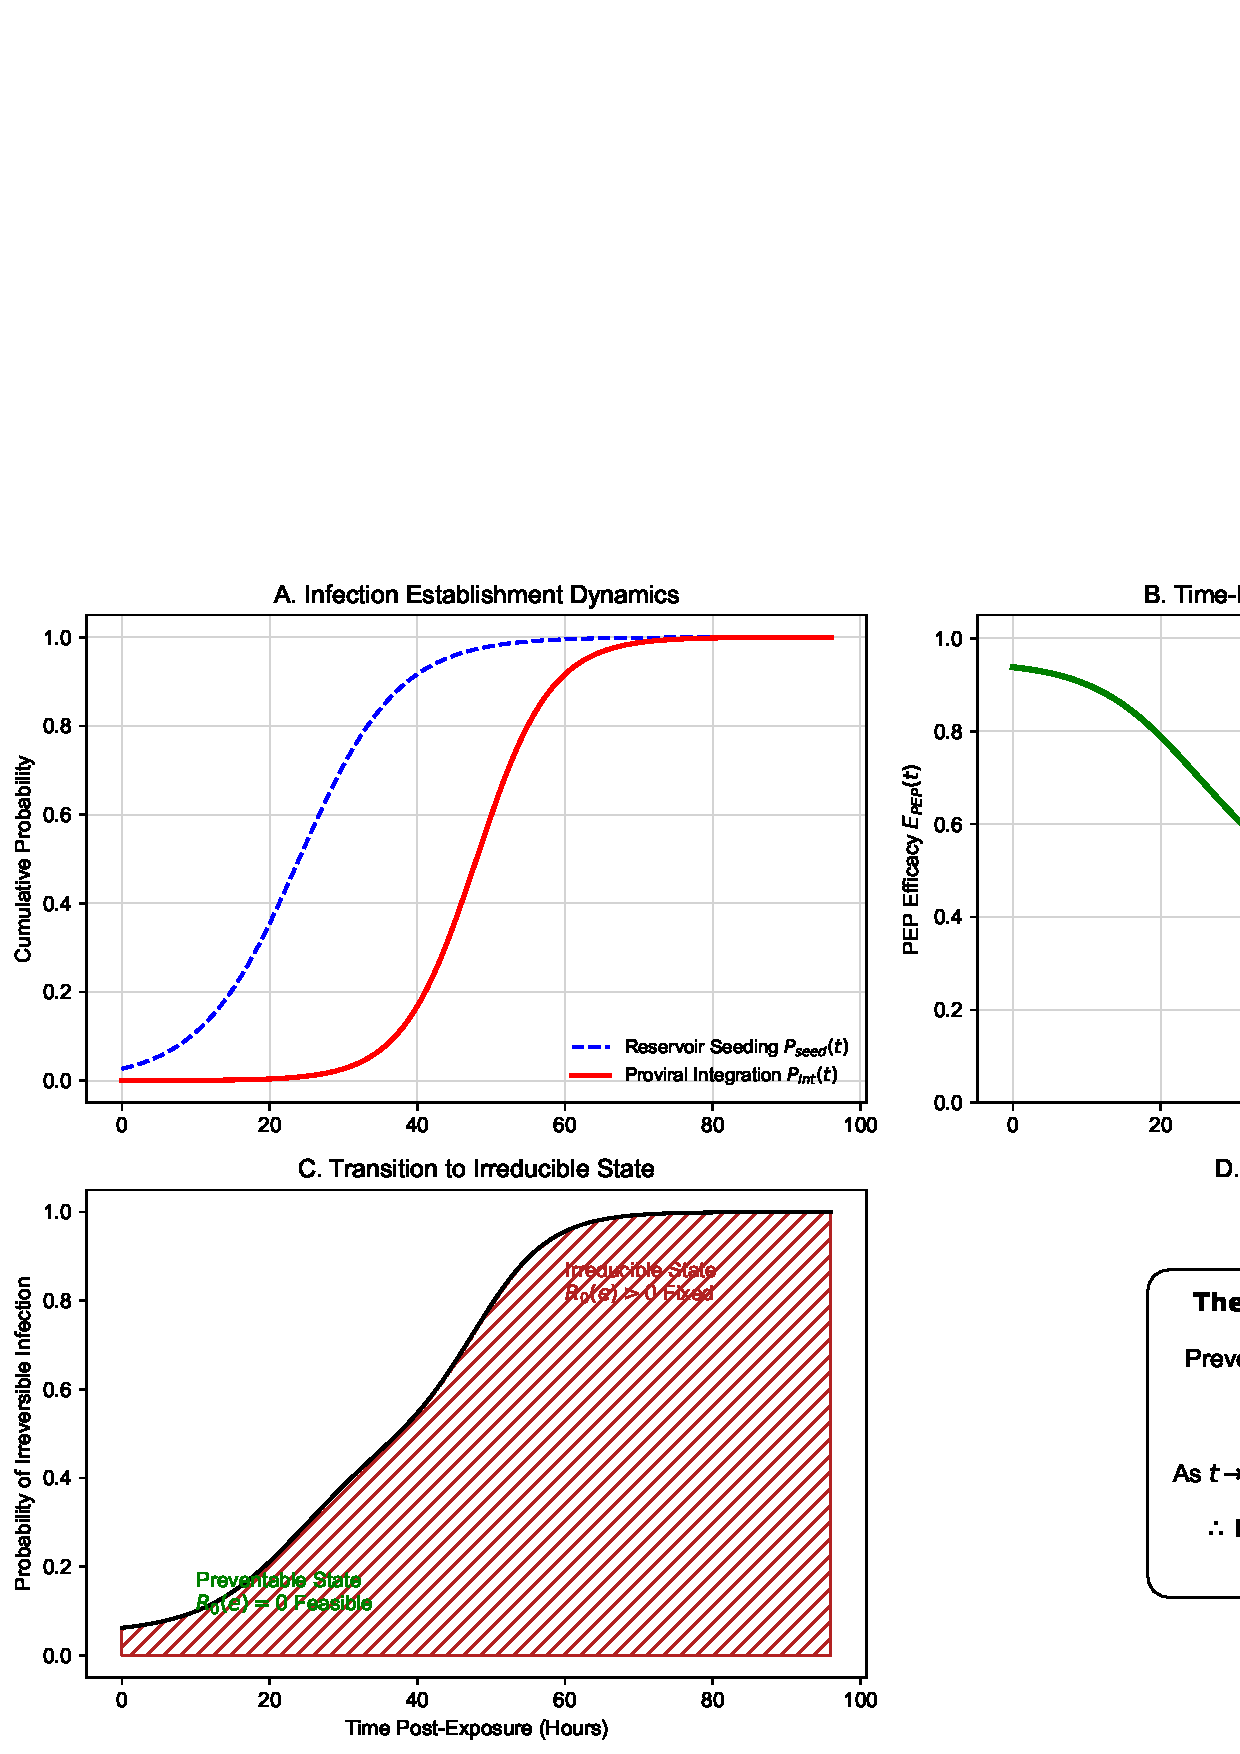
\includegraphics[width=0.95\textwidth]{Figure_1_Prevention_Theorem_Dynamics.pdf}
\caption{\textbf{The Prevention Theorem: Dynamics of Infection Establishment and Post-Exposure Prevention.} 
Panel A shows cumulative probabilities of reservoir seeding (dashed blue) and proviral integration (solid red) over time. Panel B displays the time-dependent efficacy function $E_{\mathrm{PEP}}(t)$, which decays as integration progresses. Panel C illustrates the transition from preventable to irreducible states, with the green zone representing the window during which $R_0(e)=0$ is achievable and the red zone representing the irreducible infection state. Panel D restates the theorem: prevention requires $R_0(e)=0$, which is only achievable while $P_{\text{int}}(t) < 1$.}
\label{fig:theorem}
\end{figure}

\subsection{Finite Prevention Window for Post-Exposure Prophylaxis}

Model parameterization indicates that the window for enforcing $R_0(e)=0$ extends to approximately 72 hours for mucosal exposures, constrained by local immune bottlenecks \cite{tanner_npep_2025}. However, for parenteral exposures (e.g., injection), this window is compressed to roughly 12--24 hours due to the bypass of early mucosal barriers and rapid systemic dissemination \cite{strathdee_preventing_2020}. This ``left-shift'' of the critical window significantly reduces the timeframe for effective intervention.

Figure \ref{fig:window} demonstrates the quantitative compression of the prevention window between mucosal and parenteral exposures. The parenteral route (red dashed line) shows a precipitous decline in prevention efficacy within the first 24 hours, whereas the mucosal route (blue solid line) maintains higher efficacy through 72 hours. This differential is driven by the distinct immunological bottlenecks encountered in each tissue compartment.

\begin{figure}[!htbp]
\centering
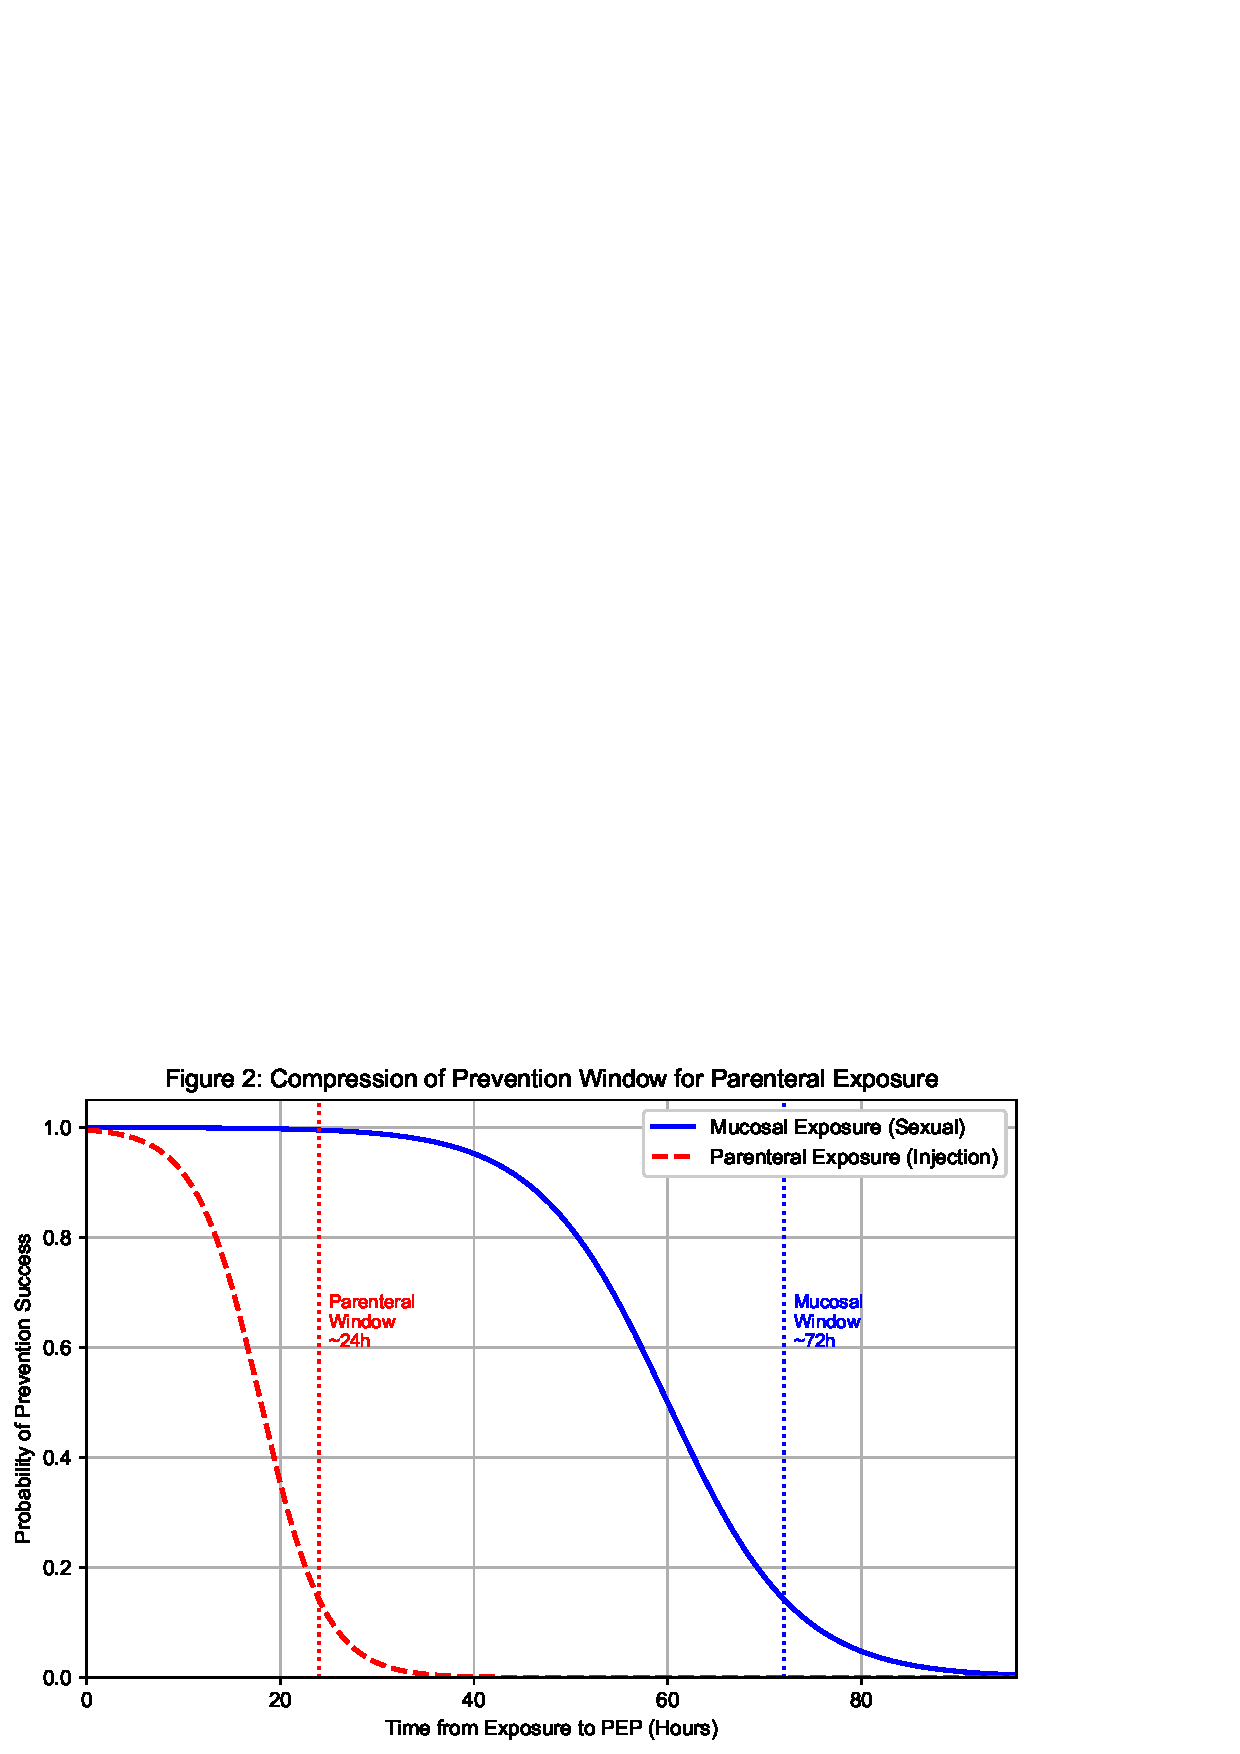
\includegraphics[width=0.85\textwidth]{Figure_2_Window_Compression.pdf}
\caption{\textbf{Compression of the Prevention Window for Parenteral Exposure.}
The solid blue line shows the probability of prevention success following mucosal exposure, which remains effective through approximately 72 hours. The dashed red line shows the dramatically compressed window for parenteral exposure, with prevention efficacy approaching zero by 24 hours. The differential reflects the bypass of mucosal immune barriers in systemic exposures, allowing more rapid establishment of productive infection.}
\label{fig:window}
\end{figure}

\subsection{Irreducible Infection State}

Proviral integration represents a thermodynamically irreversible transformation of the host genome. Once integrated, viral DNA persists for the lifetime of the cell and is propagated to all daughter cells during division, producing clonal expansion independent of ongoing viral replication \cite{wahl_hiv_2023}.

\begin{equation}
G(t+1) = G(t) + \text{HIV}_{\text{provirus}}
\end{equation}

No biologically realizable inverse transformation exists that restores the pre-integration genomic state. Consequently, once integration occurs, the condition $R_0(e)=0$ is mathematically unattainable \cite{brown_long-term_2019, hutter_long-term_2009}.

\subsection{Reservoir Stratification}

Long-lived viral reservoirs persist in specific cellular compartments, including naïve T-cells, central memory T-cells ($T_{CM}$), stem cell-like memory T-cells ($T_{SCM}$), and microglial cells \cite{wahl_hiv_2023, anderson_neuroinflammation_2020}. These compartments are characterized by self-renewal capacity and longevity, allowing viral persistence independent of viral replication \cite{hellmuth_very_2018}.

\subsection{Applied Example: Structural Infeasibility Under Access Delays}

Comparison of the derived biological windows against empirically observed access delays in high-risk populations (e.g., people who inject drugs) reveals a fundamental mismatch. Surveillance data indicates that while 85\% of sexual exposure cases present to Emergency Departments within 72 hours, structural delays for injection-related exposures consistently exceed the compressed 24-hour parenteral window \cite{taylor_stuck_2019, baugher_ending_2025}. 

For this population, the cycle time required to navigate arrest, withdrawal, and housing instability ($T_{struct}$) almost invariably exceeds the biological cycle time ($T_{bio}$). Consequently, the condition $R_0(e)=0$ is biologically unreachable before access is even attempted. In these scenarios, failure is not a probabilistic outcome of drug efficacy or adherence, but a deterministic result of timing constraints.

\section{Discussion}

\subsection{Theoretical Implications}

Prevention is fundamentally an existence problem: does a state $R_0(e)=0$ exist and is it reachable? Our analysis shows that PEP failure often represents a boundary violation rather than adherence failure; late intervention cannot alter the initial condition $R(0)>0$ once it has been established \cite{grant_evidence_1987}.

\subsection{Biological Proof of Concept: CCR5-\texorpdfstring{$\Delta$32}{Delta32}}

The only known ``cure'' scenarios involve CCR5-$\Delta$32 transplantation, which effectively eliminates the susceptibility term in the transmission equation \cite{hutter_long-term_2009}:

\begin{equation}
\frac{dR}{dt} = \lambda S V \cdot 0 = 0
\end{equation}

This intervention functions as a system replacement rather than a reversal of the infection state, reinforcing the irreversibility of the integrated provirus in susceptible hosts.

\subsection{Implications for Epidemic Control}

Reactive interventions cannot achieve epidemic control when biological establishment precedes access. Prevention architectures must therefore be evaluated against biological feasibility constraints, not solely pharmacological efficacy \cite{palella_declining_1998}.

\section{Future Work}

Future analyses will explore stochastic population dynamics and network-level avoidance collapse resulting from these constraints. The specific impact of architectural failure on population-level incidence is explicitly deferred to subsequent analysis.

%% --- BIBLIOGRAPHY ---
%\bibliographystyle{spmpsci}
\bibliography{prevention_theorem_clean}


\section*{Data Sharing}

All model code, simulation outputs, and analysis scripts are available at \url{https://github.com/Nyx-Dynamics/Prevention-Theorem}. 
All model inputs derive from published literature or synthetic populations; no individual-level data were used.

\section*{Declaration of Interests}

The author reports prior employment with Gilead Sciences, Inc. from January 2020 through
November 2024 and prior ownership of company stock, which was fully divested in December
2024. Gilead Sciences, Inc. had no role in the conception, design, analysis, interpretation, or
writing of this study, and provided no funding, data, materials, or input into any aspect of the
work.

The author is the owner of Nyx Dynamics, LLC, a consulting company providing advisory and
fractional leadership services in healthcare, technology, and complex systems. This research
was conducted independently, released as open-source work, and was not produced as part
of, or in support of, any paid consulting engagement.

No other competing interests are declared.

\section*{Ethics Approval and Consent to Participate}

This study did not involve human participants, human biological samples, or the collection of
identifiable private information. All analyses were conducted using publicly available,
aggregate data from published literature and guidelines. As such, institutional review board
(IRB) approval and informed consent were not required.
\section*{Acknowledgments}

\textbf{Communities.}
The author thanks the HIV prevention research community whose published work informed model
parameterization, and the people who inject drugs (PWID) community advocates whose testimony
informed characterization of structural barriers.

\textbf{Use of Artificial Intelligence and Assistive Technologies.}
The author acknowledges the use of artificial intelligence–assisted tools during manuscript
preparation. Computational analyses were conducted using Python with open-source packages
including NumPy, Pandas, SciPy, Matplotlib, and Seaborn. Large language models (Anthropic
Claude and OpenAI ChatGPT) were used to support literature search and improve readability of
the manuscript. JetBrains Junie was used for code correction, and Zotero AI was used for
reference management. Manuscript preparation was conducted using the Overleaf \LaTeX{}
platform. All AI tools were used as assistive technologies only. The author retains full
responsibility for study design, data analysis, interpretation of results, and all conclusions
presented.

\end{document}




